\section{Transformatorn}
\textbf{HAREC a.\ref{HAREC.a.2.4}\label{myHAREC.a.2.4}}
\label{transformator}
\label{primärlindning}
\label{transformator!primärlindning}
\label{sekundärlindning}
\label{transformator!sekundärlindning}

\subsection{Allmänt}

En \emph{transformator} (eng. \emph{transformer}) består av en eller flera
lindningar eller spolar av elektriska ledare.
Lindningarna är magnetiskt kopplade till varandra.
Det innebär att de är anordnade så att ett magnetfält som alstrats i någon
av lindningarna även passerar genom övriga lindningar.

När en växelspänning läggs över en lindning kallas den \emph{primärlindning}
(eng. \emph{primary coil}).
I och omkring primärlindningen alstras då ett magnetiskt fält som växlar i takt
med spänningen. Primärfältet passerar även genom övriga lindningar --
\emph{sekundärlindningarna} (eng. \emph{secondary coil}) -- och alstrar där
spänningar och strömmar.

Den så kallade kopplingsfaktorn mellan lindningarna varierar för olika frekvenser. 
Den är lägre vid låga frekvenser (hundratals Hz) och högre vid höga frekvenser
(tusentals Hz).
Speciellt vid låga frekvenser behövs en större kopplingsfaktor för att avsedd
effekt ska kunna överföras mellan lindningarna. Då kan ledningsförmågan i den
magnetiska flödesvägen ökas med hjälp av en järnkärna.

\begin{figure}[ht]
%  \begin{mdframed}
    \begin{center}
      \begin{circuitikz}
        \draw
        (1,1) node[transformer](T1) {}
        (T1.base) node{1}
        ;
        \draw[european]
        (4,1) node[transformer](T2) {}
        (T2.base) node{2}
        ;
        \draw
        (7,1) node[transformer core](T3) {}
        (T3.base) node{3}
        ;
      \end{circuitikz}
      \\
      \begin{tabular}{ll}
        1, 2 & Allmänna symboler \\
        3 & Transformator med kärna
      \end{tabular}
    \end{center}
    \caption{Schemasymboler för transformatorer}
%  \end{mdframed}
  \label{fig:BildII2-5}
\end{figure}

Bild \ref{fig:BildII2-5} illustrerar flera vanligt förekommande schemasymboler
för transformatorer med två lindningar.

\subsection{Utföranden}
\index{spänningstransformator}
\index{transformator!spännings-}
\index{strömtransformator}
\index{transformator!ström-}
\index{impedanstransformator}
\index{transformator!impedans-}

Transformatorn kan utföras för olika ändamål, till exempel som
\emph{spänningstransformator} (eng. \emph{voltage transformer}),
\emph{strömtransformator} (eng. \emph{current transformer}) eller
\emph{impedanstransformator} (eng. \emph{impedance transformer}).

Utförandet påverkas även av frekvens och av vilken effekt som ska överföras.

\subsection{Terminologi}
\index{varvtalsomsättning}
\index{transformator!varvtalsomsättning}
\index{impedansomsättning}
\index{transformator!impedansomsättning}

\begin{tabular}{ll}
primärkrets & sekundärkrets \\
primärlindning & sekundärlindning \\
primärspänning \(u_1\) &  sekundärspänning \(u_2\) \\
primärström \(i_1\) & sekundärström \(i_2\) \\
lindningsvarvtal n & primärt \(n_1\) sekundärt \(n_2\)
\end{tabular}

varvtalsomsättning = \(\dfrac{n_1}{n_2}\) eller \(\dfrac{n_2}{n_1}\)

impedansomsättning = \(\dfrac{Z_1}{Z_2}\) eller \(\dfrac{Z_2}{Z_1}\)

\subsection{Den ideala (förlustfria) transformatorn}
\textbf{HAREC a.\ref{HAREC.a.2.4.1}, a.\ref{HAREC.a.2.4.2.1},
a.\ref{HAREC.a.2.4.2.2}\label{myHAREC.a.2.4.1}
\label{myHAREC.a.2.4.2.1}\label{myHAREC.a.2.4.2.2}}
\index{varvtalsomsättning}
\index{transformator!varvtalsomsättning}
\index{impedansomsättning}
\index{transformator!impedansomsättning}

\begin{figure*}[ht]
\begin{center}
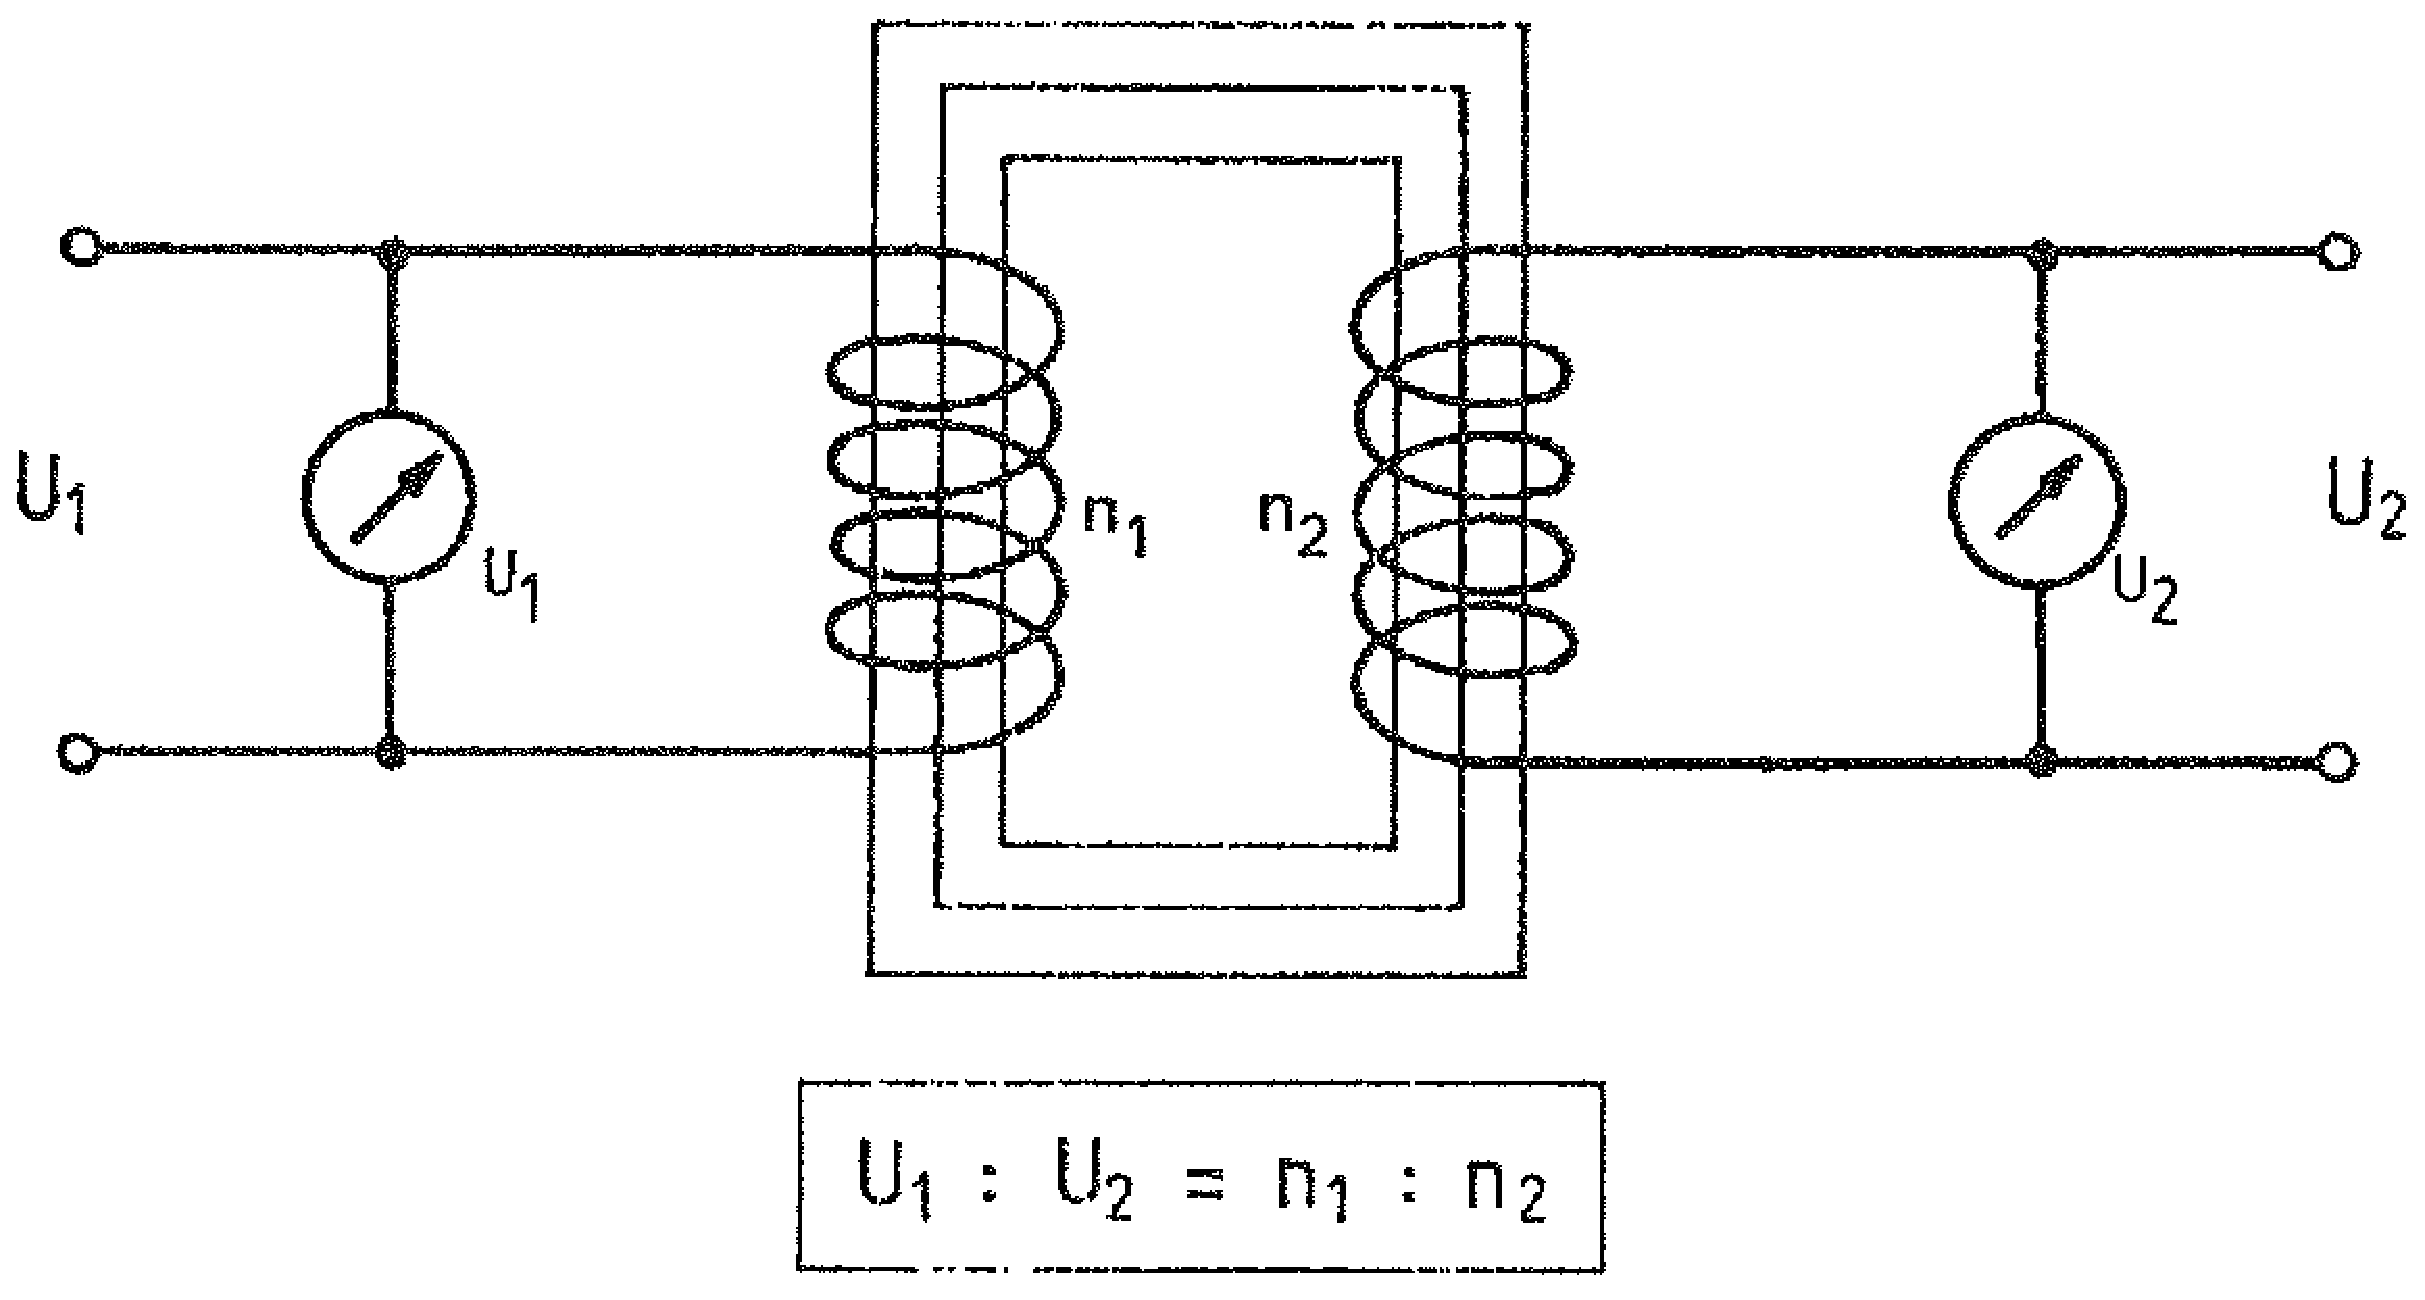
\includegraphics[width=\textwidth]{images/cropped_pdfs/bild_2_2-06.pdf}
\caption{Obelastad transformator}
\label{fig:BildII2-6}
\end{center}
\end{figure*}

I bild \ref{fig:BildII2-6} är transformatorn är obelastad när sekundärkretsen
är bruten.

När primärlindningen ansluts till en växelspänning induceras växelspänningar 
både över primär- och sekundärlindningarna. Det uppstår även en ström i 
primärlindningen, men däremot inte i sekundärlindningen när
sekundärkretsen är bruten. För den obelastade transformatorn gäller sambandet

\(\dfrac{u_1}{u_2} = \dfrac{n_1}{n_2}\)

det vill säga att spänningen över lindningarna är proportionell mot lindningsvarvtalen.

\begin{figure*}[ht]
\begin{center}
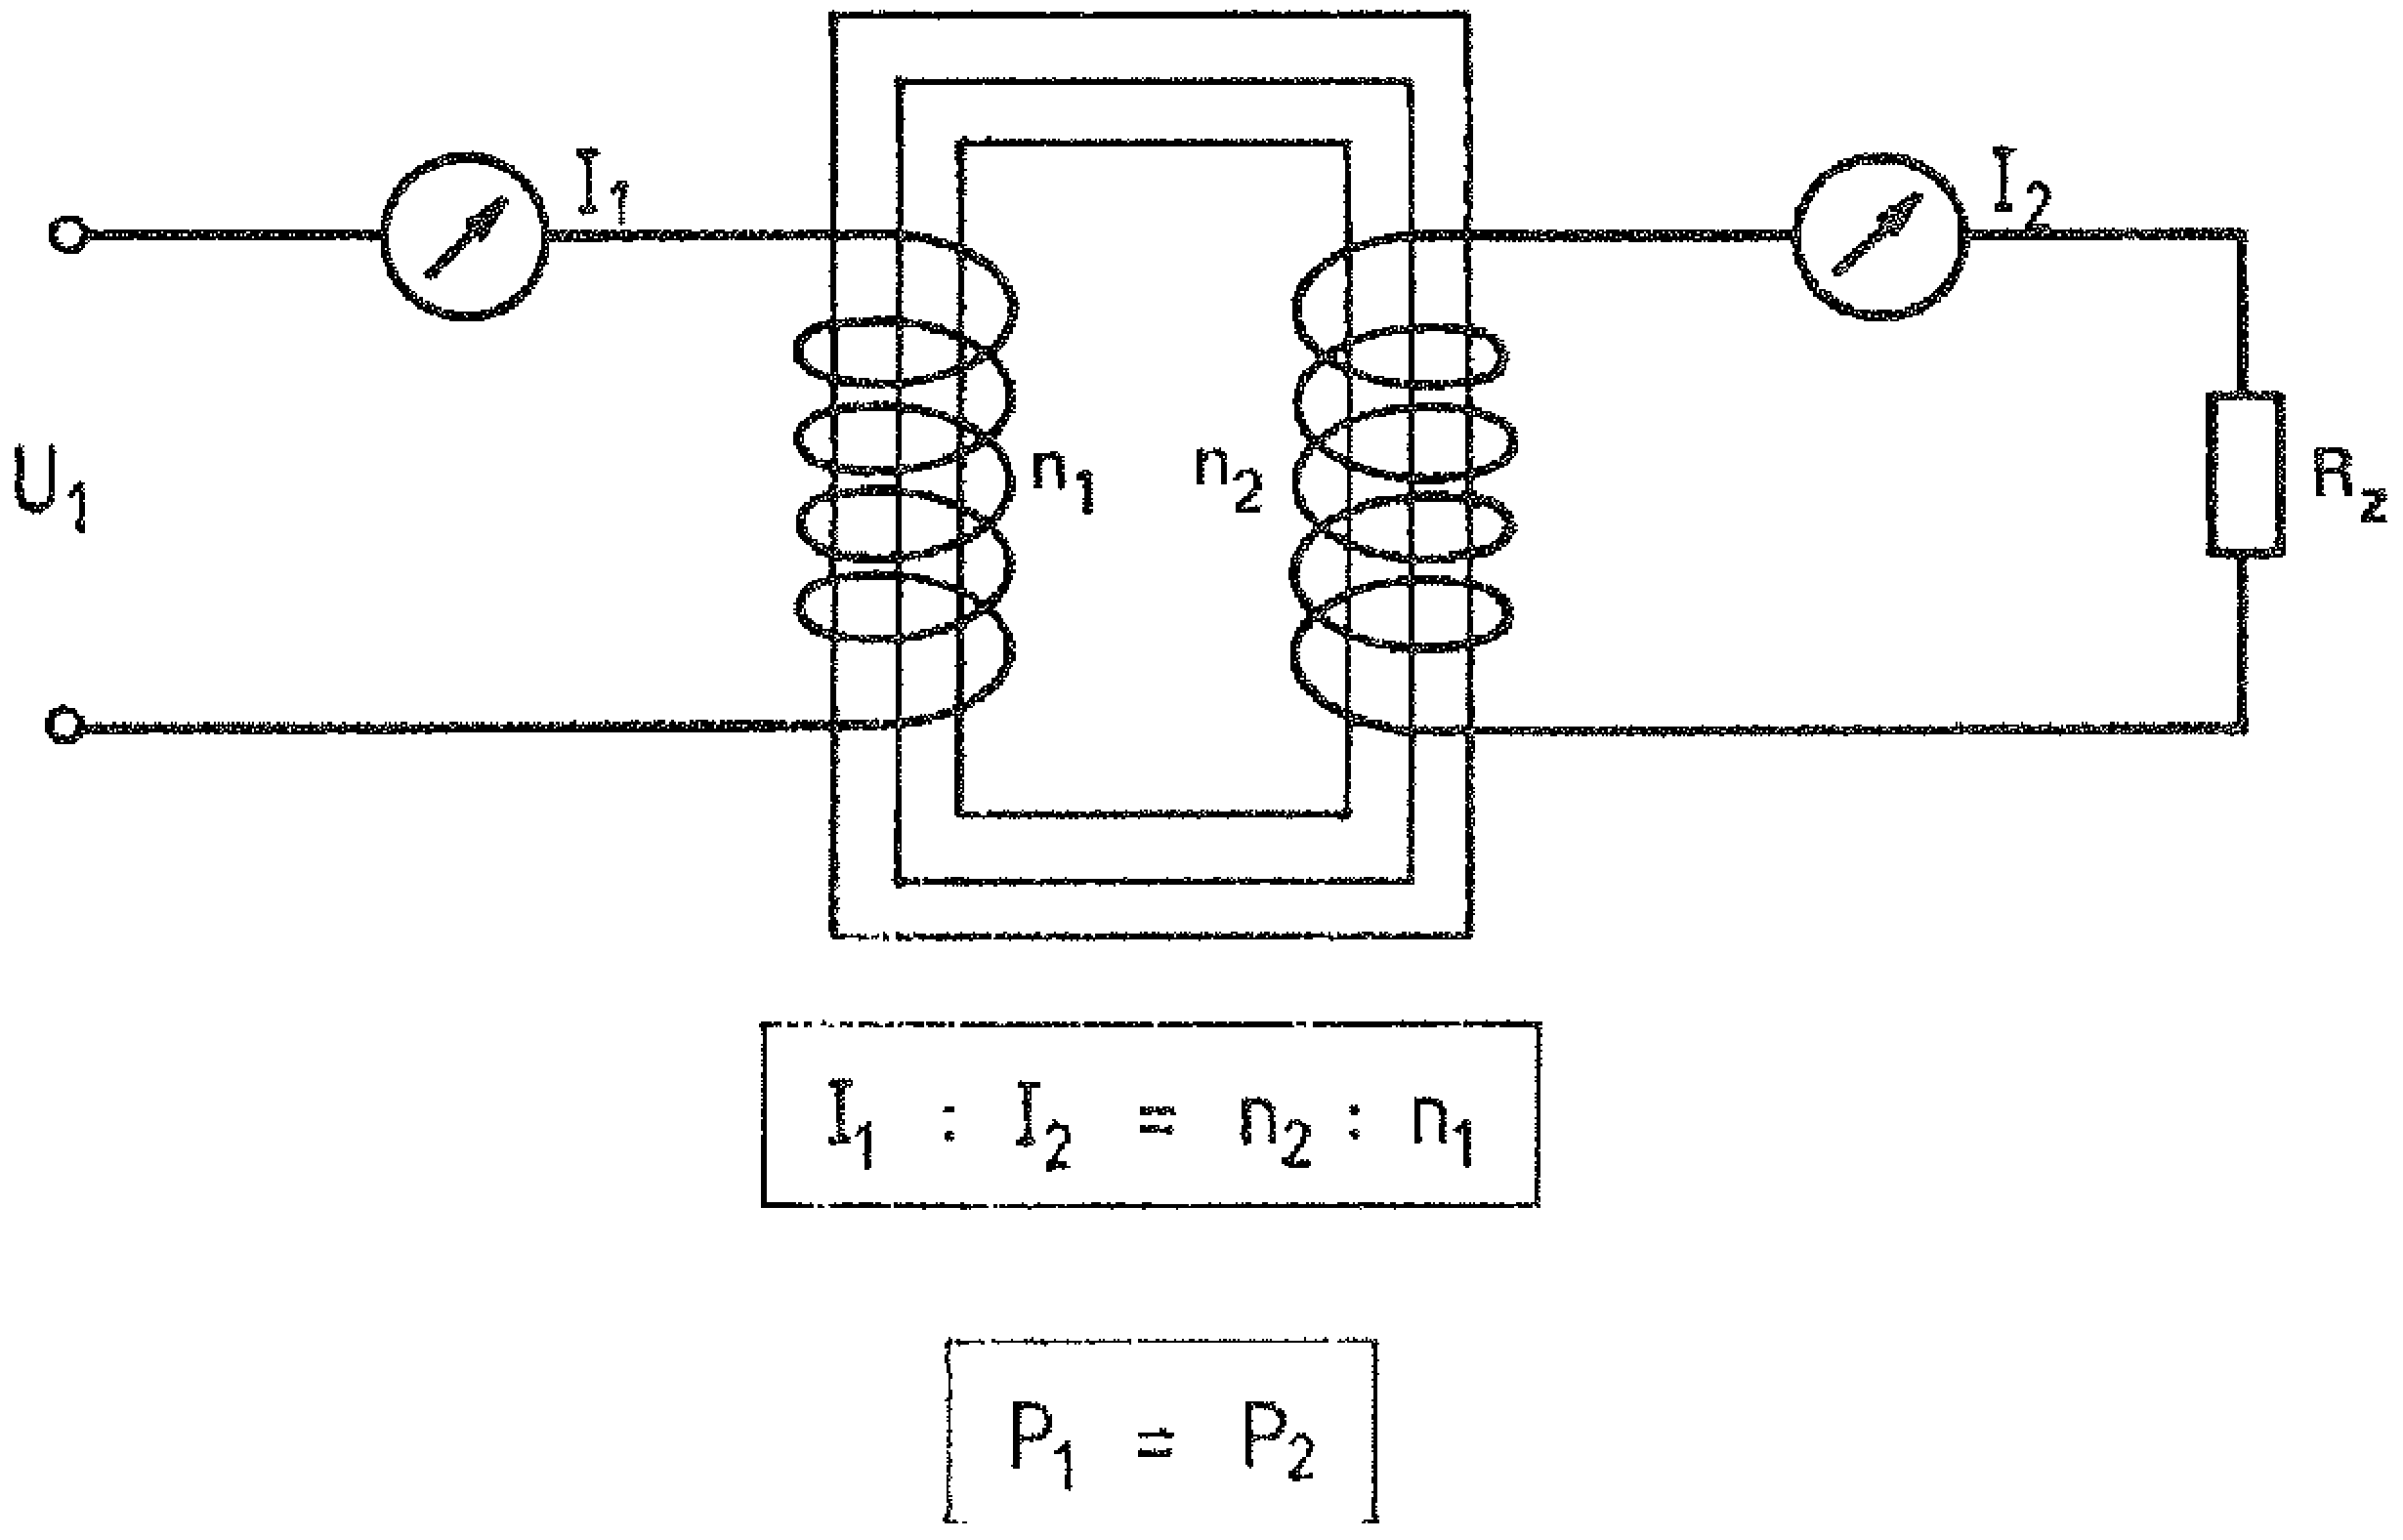
\includegraphics[width=\textwidth]{images/cropped_pdfs/bild_2_2-07.pdf}
\caption{Belastad transformator}
\label{fig:BildII2-7}
\end{center}
\end{figure*}

I bild \ref{fig:BildII2-7} är transformatorn belastad när sekundärkretsen
är sluten.

När någon av transformatorns sekundärlindningar ingår i en sluten strömkrets 
uppstår en sekundärström där.

Sekundärströmmen alstrar ett magnetfält som motverkar primärströmmens fält,
hindrar dess växlingar och tar ut energi från primärkretsen.

Strömförbrukningen på primärsidan ökar således i proportion mot
strömförbrukningen på sekundärsidan. Transformatorn reglerar själv hur mycket
energi som den tar från strömkällan och lagrar i fältet för att föra över
till sekundärkretsen.

För den belastade transformatorn gäller att strömmen genom lindningarna är
omvänt proportionell mot lindningsvarvtalet, det vill säga omvänt proportionell 
mot varvtalsomsättningen.

\(\dfrac{i_1}{i_2} = \dfrac{n_2}{n_1}\)

Av föregående formler följer att:

\(\dfrac{u_1}{u_2} = \dfrac{i_2}{i_1}\)

Av \(P_1 = u_1 \cdot i_1\) och \(P_2 = u_2 \cdot i_2\) följer att \(P_1 = P_2\).

Om man bortser från förlusterna i transformatorn, är den effekt som den tar
från kraftkällan lika med den effekt som transfromatorn avger.

Eftersom transformatorn transformerar både spänningar och strömmar, kommer
även impedansen att transformeras genom transformatorn.
Denna impedanstransformation följer impedansomsättningen, det vill säga

\(\dfrac{Z_1}{Z_2} = \dfrac{n_1^2}{i_2^2}\)

\subsection{Transformatortillämpningar}
\textbf{HAREC a.\ref{HAREC.a.2.4.2.4}\label{myHAREC.a.2.4.2.4}}

\subsubsection{Sparkopplade transformatorer}
\index{galvanisk förbindelse}
\index{spartransformator}
\index{transformator!spar-}

\begin{figure*}[ht]
\begin{center}
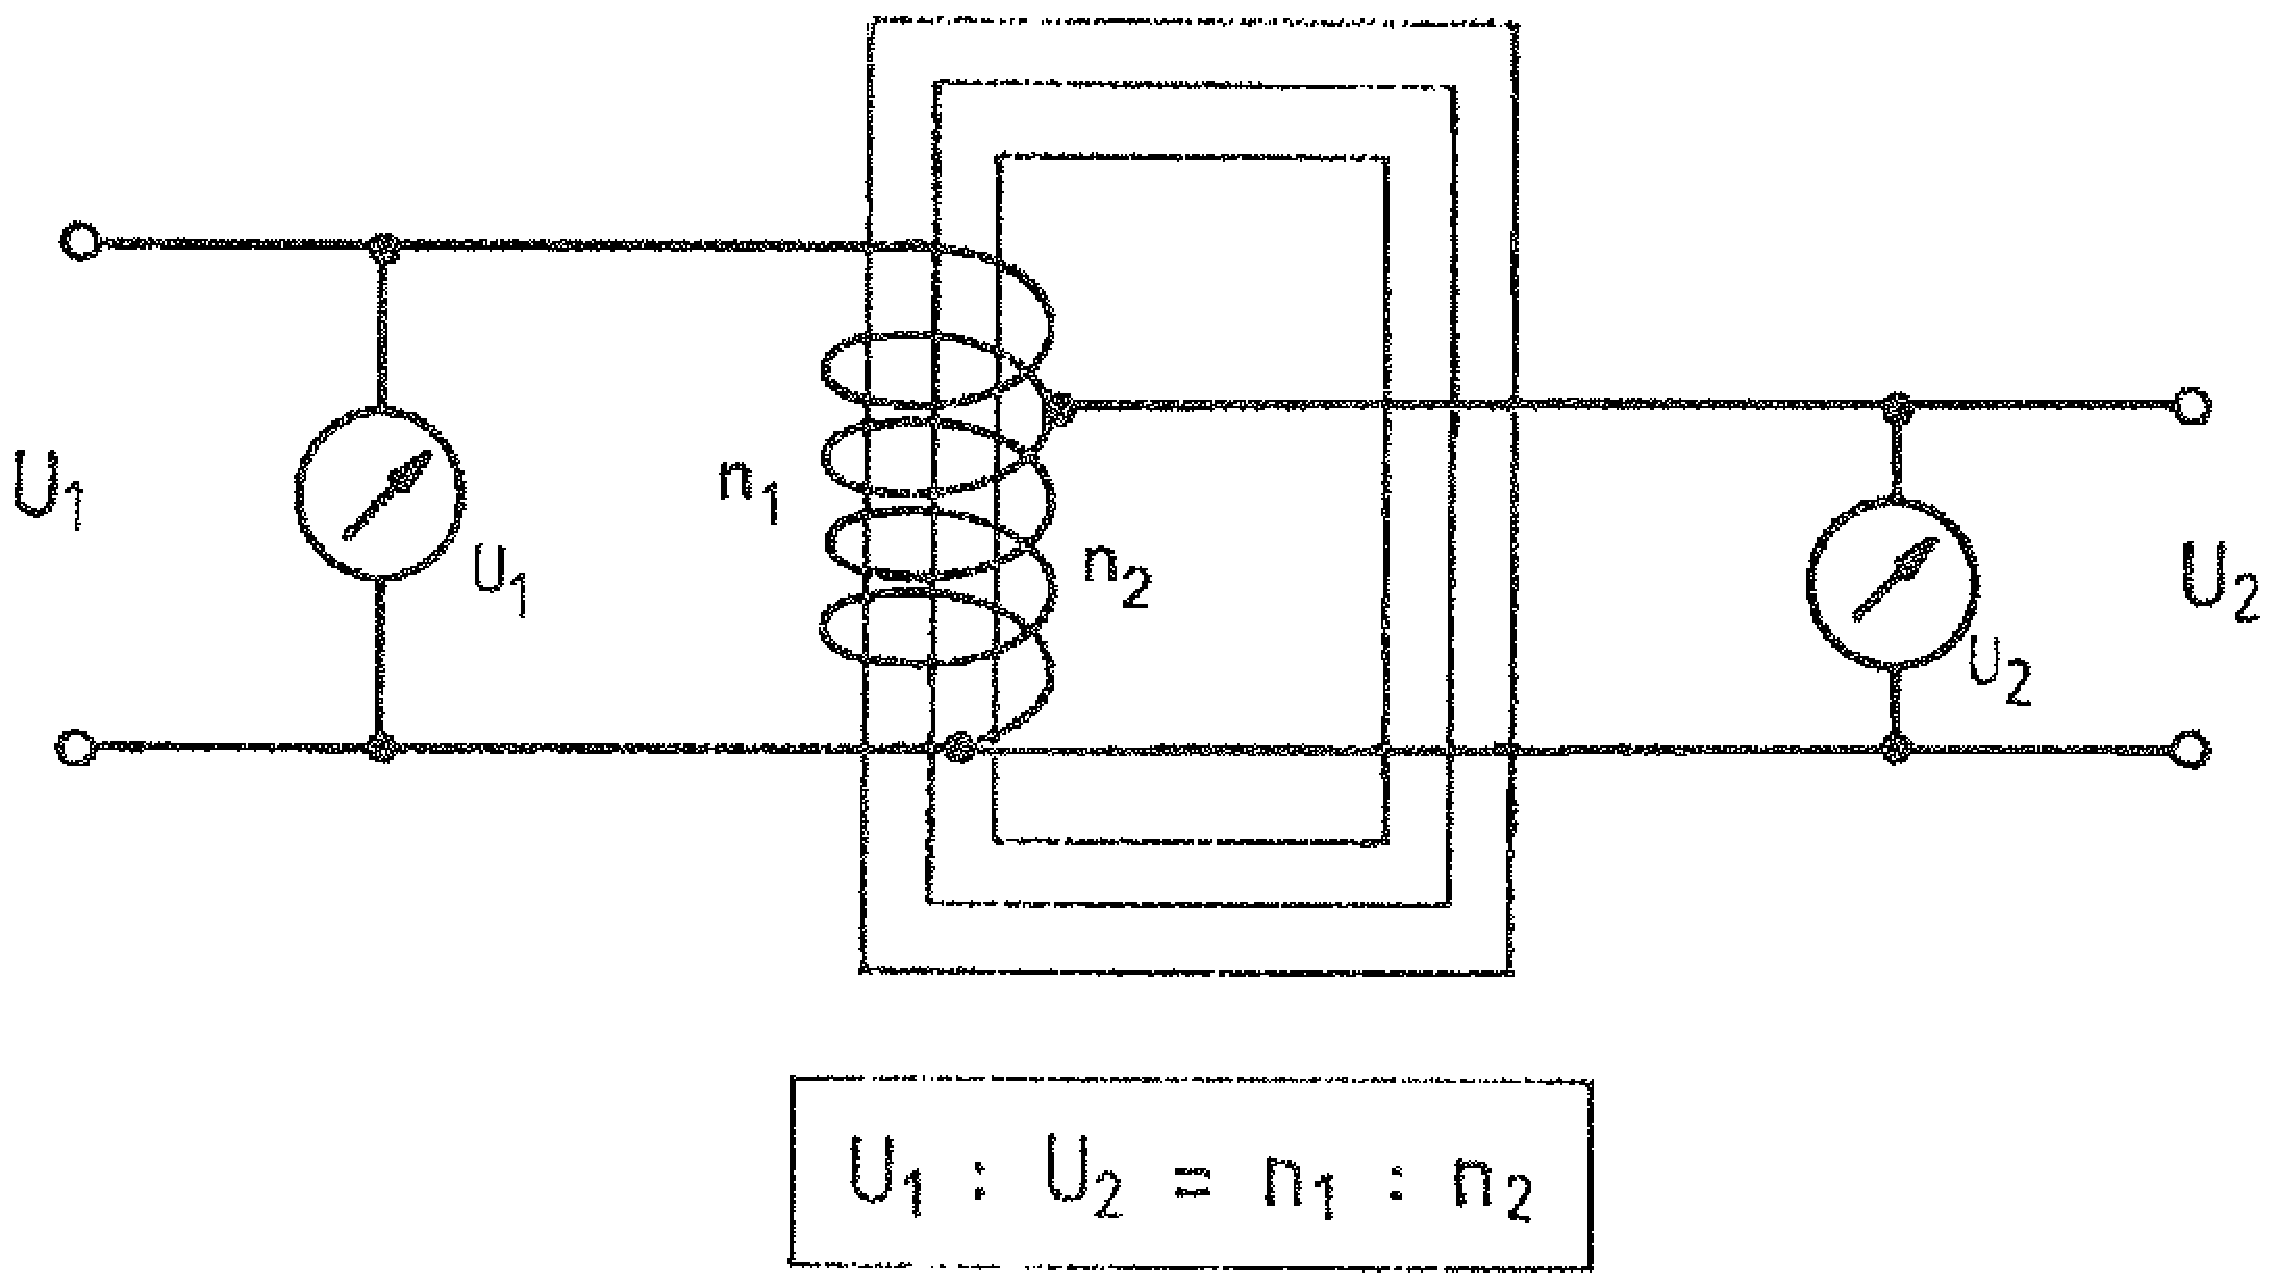
\includegraphics[width=\textwidth]{images/cropped_pdfs/bild_2_2-08.pdf}
\caption{Sparkopplad transformator}
\label{fig:BildII2-8}
\end{center}
\end{figure*}

I bild \ref{fig:BildII2-7} har transformatorn beskrivits så att primär- och
sekundärlindningarnas enda förbindelse med varandra är över ett magnetfält,
alltså utan galvanisk förbindelse.

Varje lindning kan emellertid förses med godtyckliga uttag. Mellan uttagen finns 
då en spänning som är proportionell mot antalet lindningsvarv mellan dessa.

Detta är en metod att spara in på antalet lindningar. För att till exempel omsätta
nätspänningen 230~V till 115~V används ibland en \emph{spartransformator}.

Med en spartransformator kommer olika strömkretsar i galvanisk förbindelse med
varandra, vilket visas i bild I bild \ref{fig:BildII2-8}. Särskild försiktighet ska därför 
iakttas vid användning av sparkopplade transformatorer, på grund av risken för 
elolycksfall. Spartransformatorer bör därför inte användas i amatörradiosammanhang. 
Säkrast är skyddstransformatorer med galvaniskt skilda ledningar och dessutom 
med speciellt bra isolering och kapsling.

\subsubsection{Strömtransformatorer}
\index{strömtransformator}
\index{transformator!ström-}

Hög sekundärström under låg sekundärspänning kännetecknar en
\emph{strömtransformator} (eng. \emph{current transformer}),
som illustreras i bild \ref{fig:BildII2-9}.
Strömtransformatorer används i elektriska svetsningsutrustningar,
induktionsugnar och liknande. Strömtransformatorer används även för mätning 
av höga växelströmmar.

\begin{figure*}[ht]
\begin{center}
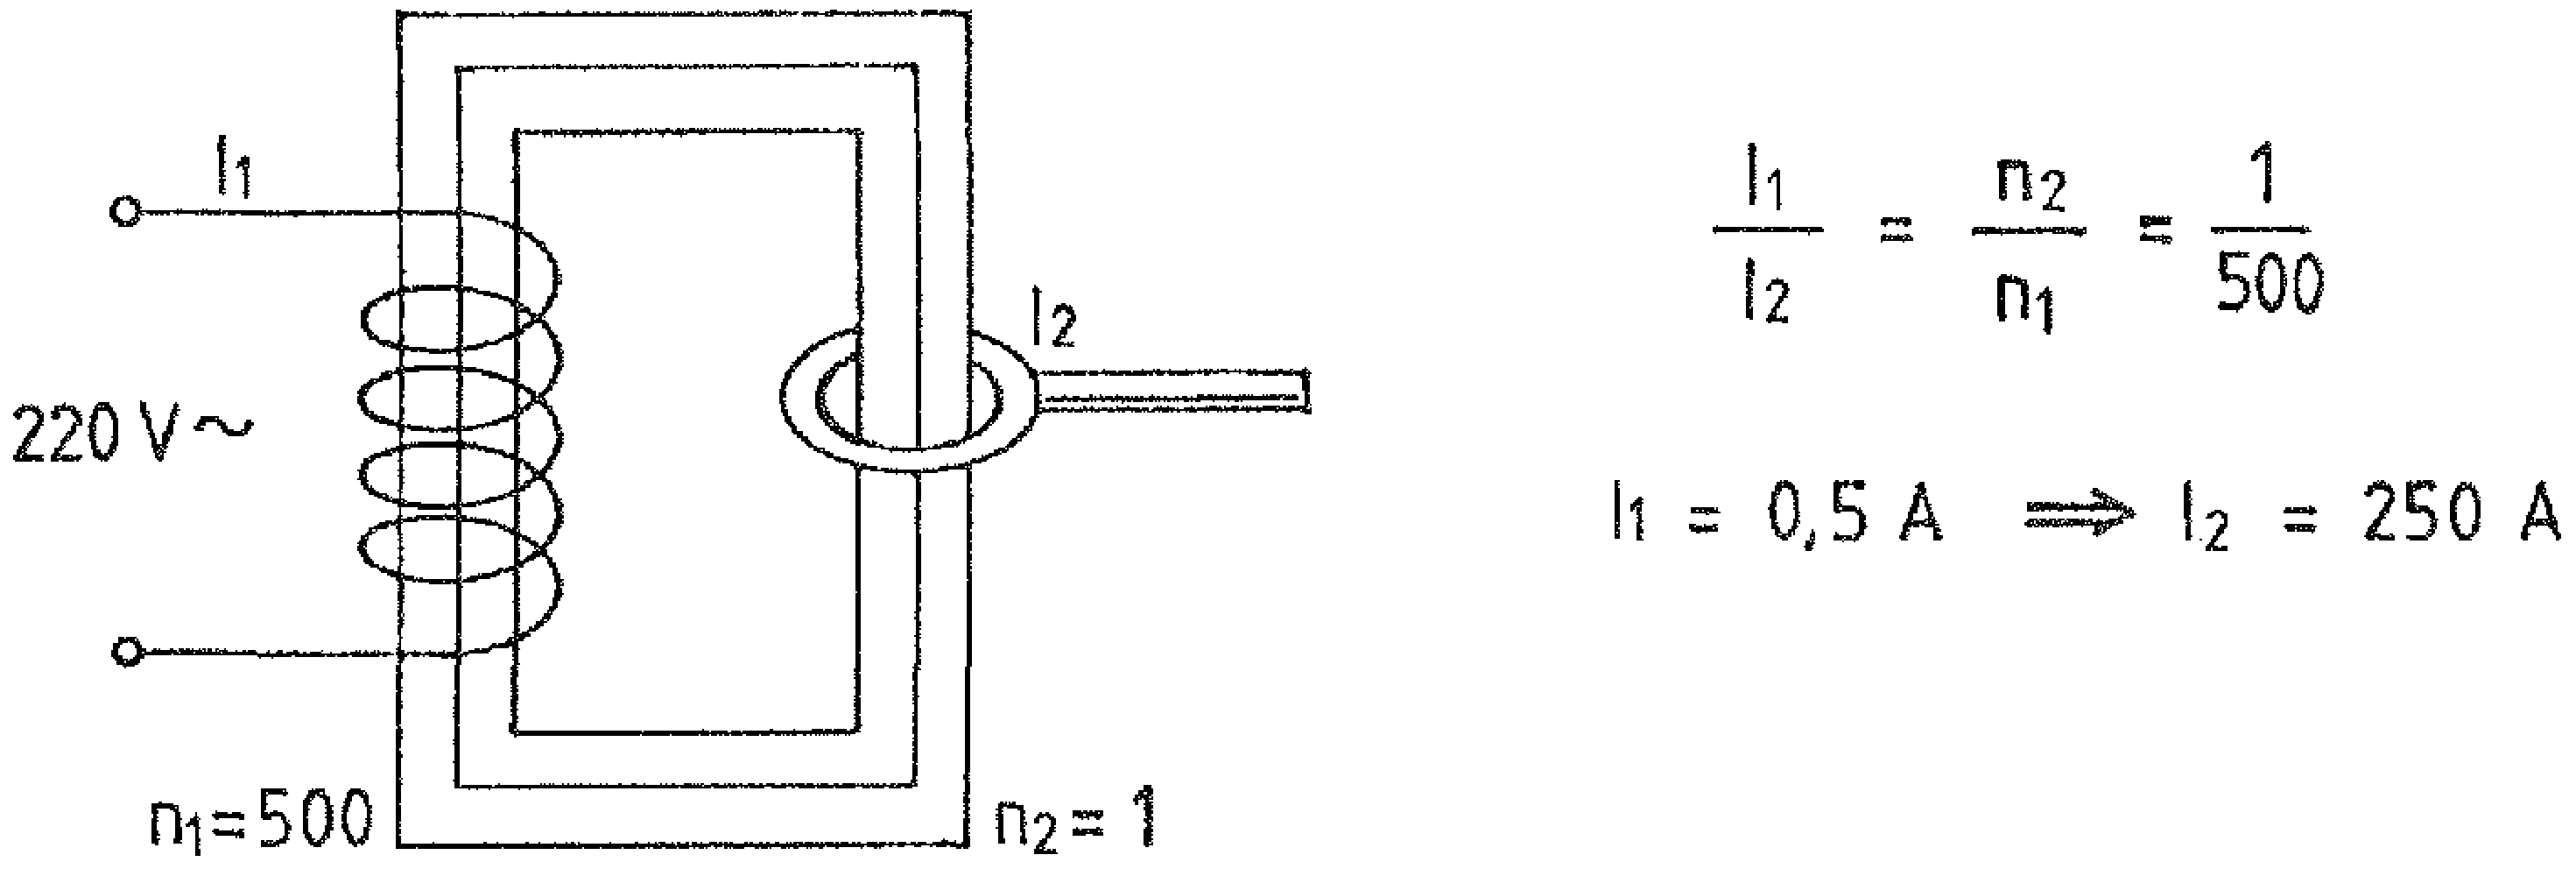
\includegraphics[width=\textwidth]{images/cropped_pdfs/bild_2_2-09.pdf}
\caption{Strömtransformator}
\label{fig:BildII2-9}
\end{center}
\end{figure*}

\subsubsection{Högspänningstransformatorer}
\index{spänningstransformator}
\index{transformator!spännings-}
\index{högspänningstransformator}
\index{transformator!högspännings-}

Hög sekundärspänning under förhållandevis låg sekundärström kännetecknar en
\emph{spänningstransformator} (eng. \emph{voltage transformer}).
Bild \ref{fig:BildII2-10} visar en transformator med ett gnistgap i
sekundärkretsen för tändning av gas.

\emph{Högspänningstransformatorer} (eng. \emph{high voltage transformer})
används i distributionsnät, neonskyltar, tändsystem för förbränningsmotorer,
anodspänningsaggregat för sändare osv.

\begin{figure*}[ht]
\begin{center}
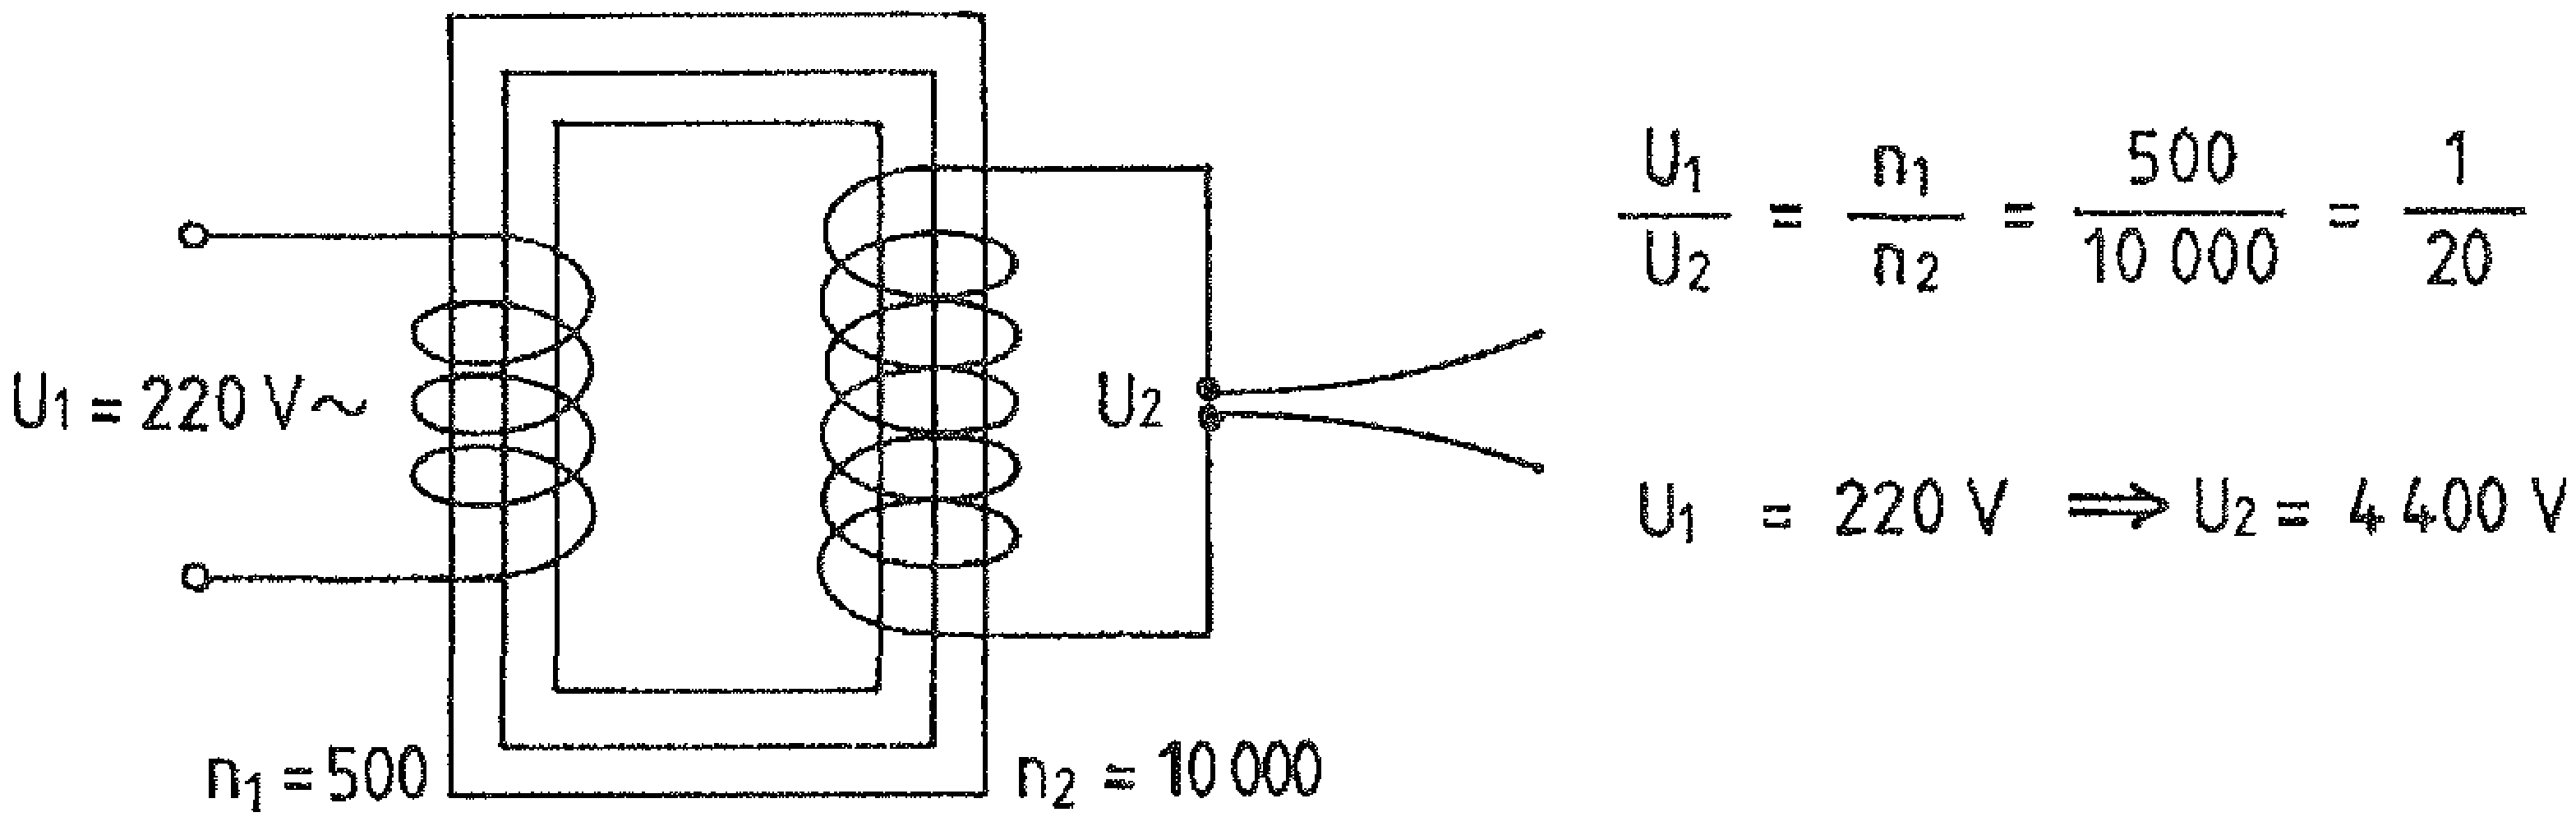
\includegraphics[width=\textwidth]{images/cropped_pdfs/bild_2_2-10.pdf}
\caption{Högspänningstransformator}
\label{fig:BildII2-10}
\end{center}
\end{figure*}

\subsubsection{Låg- och klenspänningstransformatorer}
\index{spänningstransformator}
\index{transformator!spännings-}
\index{lågspänningstransformator}
\index{transformator!lågspännings-}
\index{skyddstransformator}
\index{transformator!skydds-}

\begin{figure*}[ht]
\begin{center}
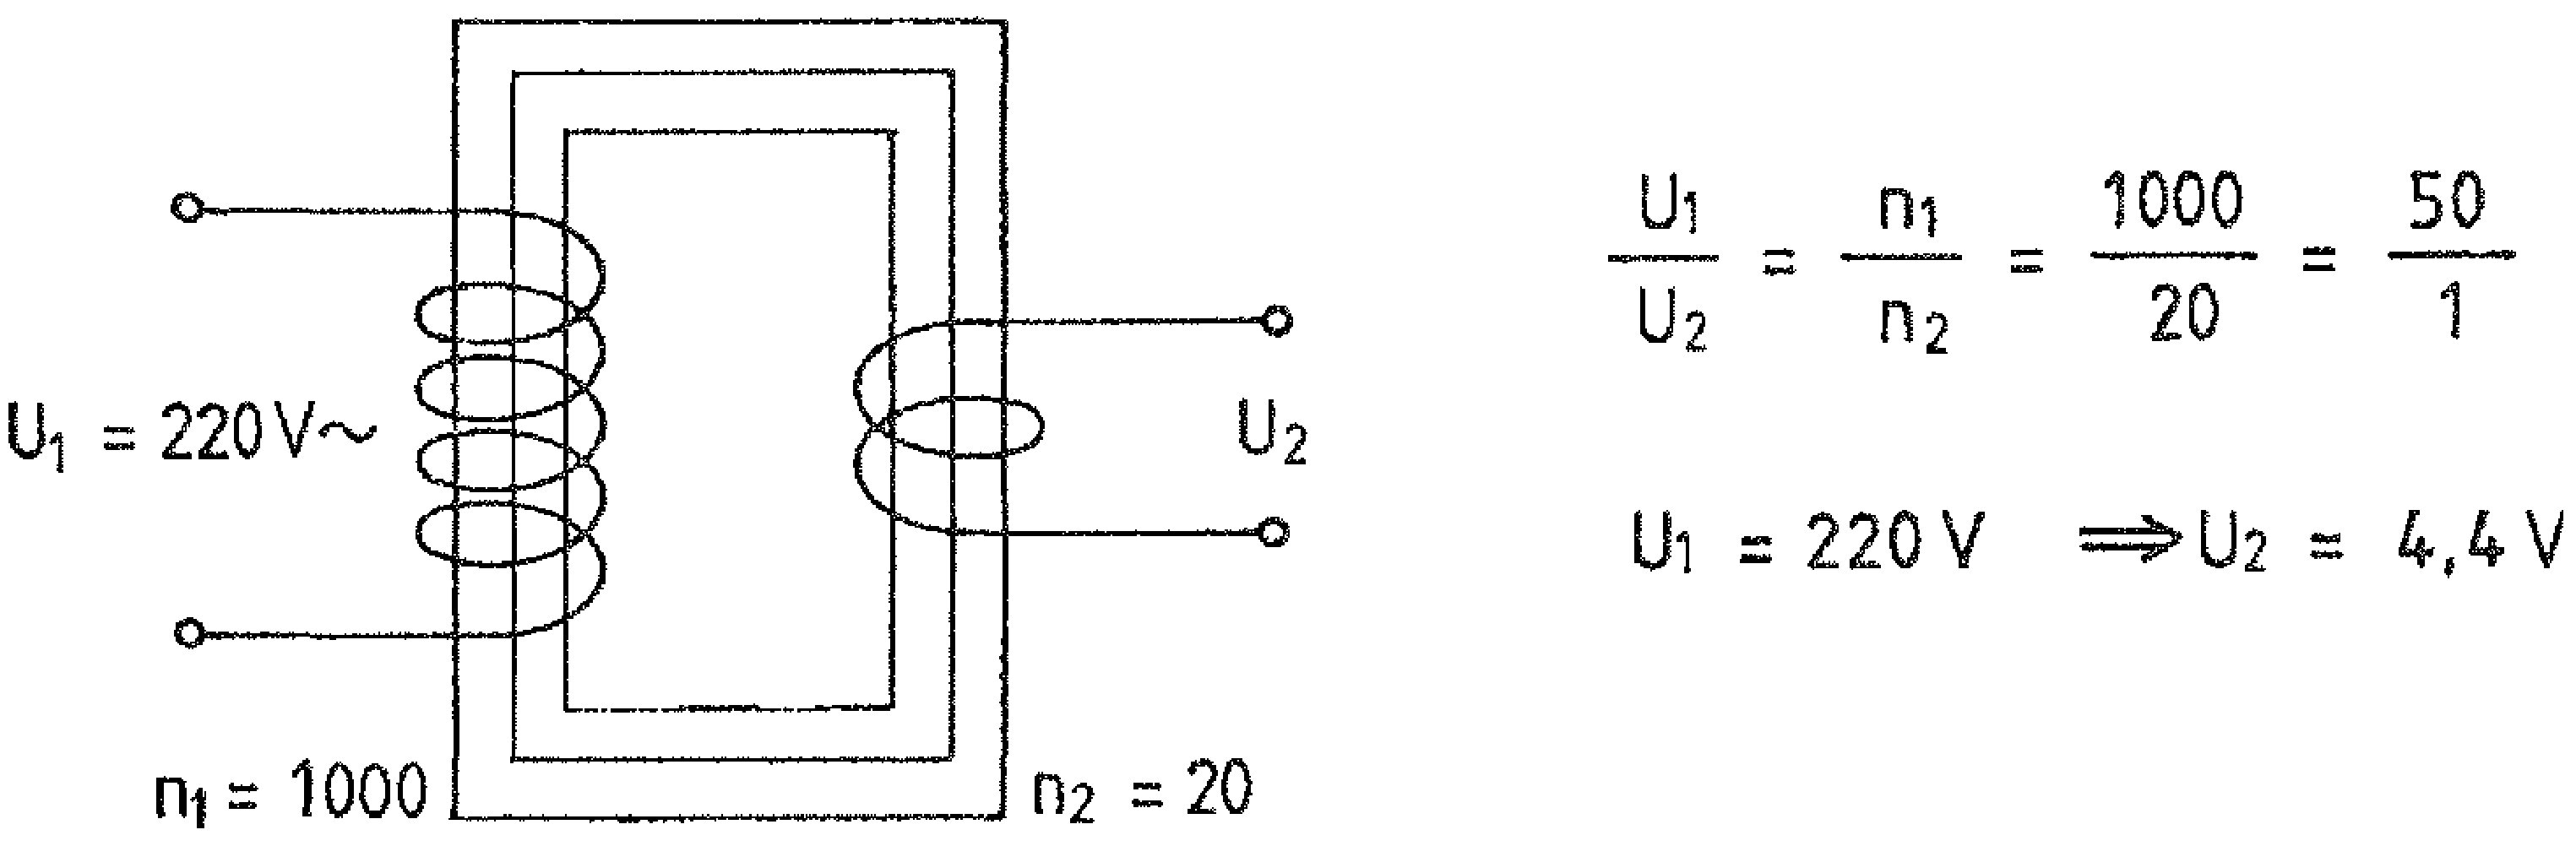
\includegraphics[width=\textwidth]{images/cropped_pdfs/bild_2_2-11.pdf}
\caption{Klenspänningstransformator}
\label{fig:BildII2-11}
\end{center}
\end{figure*}

En \emph{lågspänningstransformator} (eng. \emph{low voltage transformer}) 
med spänningen 400/230~V används i lokala distributionsnät, det vill säga de 
elektriska ledningar som går från en transformator till vanliga hus och kontor.

För ökad säkerhet mot elektrisk chock krävs dock att vissa apparater drivs med
klenspänning via en \emph{skyddstransformator}
(eng. \emph{safety isolating transformer}).
Det är en transformator med skyddsseparation mellan primär- och
sekundärlindningarna.
Sekundärspänningen i en klenspänningstransformator, bild \ref{fig:BildII2-11},
får inte överstiga 50~V.

\subsection{Sambandet mellan varvtal och impedans}
\textbf{HAREC a.\ref{HAREC.a.2.4.2.3}\label{myHAREC.a.2.4.2.3}}
\index{impedans!transformator varvtal}
\index{impedansomsättning}
\index{transformator!impedansomsättning}
\index{impedanstransformator}
\index{transformator!impedans-}

Transformatorn kan även användas för anpassning av impedanser.
Impedansen Z i en lindning är proportionell mot kvadraten av dess
lindningsvarvtal n.

Om effekten i sekundärlindningen är lika stor som i primärlindningen, gäller
formeln

\(\dfrac{Z_p}{Z_s} = \dfrac{n_p^2}{n_s^2}\)
